\documentclass{article}
\usepackage{times}
\usepackage{hyperref}
\usepackage{graphicx}
\usepackage{shorttoc}

\begin{document}

\title{The Animal Audiogram Database Administration Manual}
\author{Ortiz Troncoso A.\\ \\
  Museum f{\"u}r Naturkunde Berlin\\Leibniz-Institut f{\"u}r Evolutions- und Biodiversitätsforschung\\
  \texttt{Alvaro.OrtizTroncoso@mfn.berlin}
}
\date{Version 1.0, 8. April 2021}

\maketitle

%----------------------------------------------------------------------------------------------%
\begin{abstract}
  This is the manual for administrators of the Animal Audiograms Database (AAD). This manual documents how to create, update and delete audiograms from the database, as well as adding bibliographic references and taxonomic entries.
\end{abstract}

\tableofcontents

%----------------------------------------------------------------------------------------------%
\section{Accessing the administration interface}
The AAD is a publicly accessible ressource and can be accessed here:\\ \url{animalaudiograms.museumfuernaturkunde.berlin/}

Accessing the administration interface requires administrative privileges. Therefore, the administration interface is password-protected. Please contact your system administrator to get a password that will grant you administrative privileges.

Once you have been granted administrative privileges, access the administration interface by opening this url in a browser:\\
\url{https://animalaudiograms.museumfuernaturkunde.berlin/admin/v1/start}\\
Login with your administrative password.


% ----------------------------------------------------------------------------------------------%
\section{Edit an experiment's details}
\subsection{What are experiment details?}
Audiograms are acquired through experimental procedures. The details of the experiment are displayed in the AAD under the ``Experiment details'' tab (fig. \ref{fig:experiment_details}).

\begin{figure}
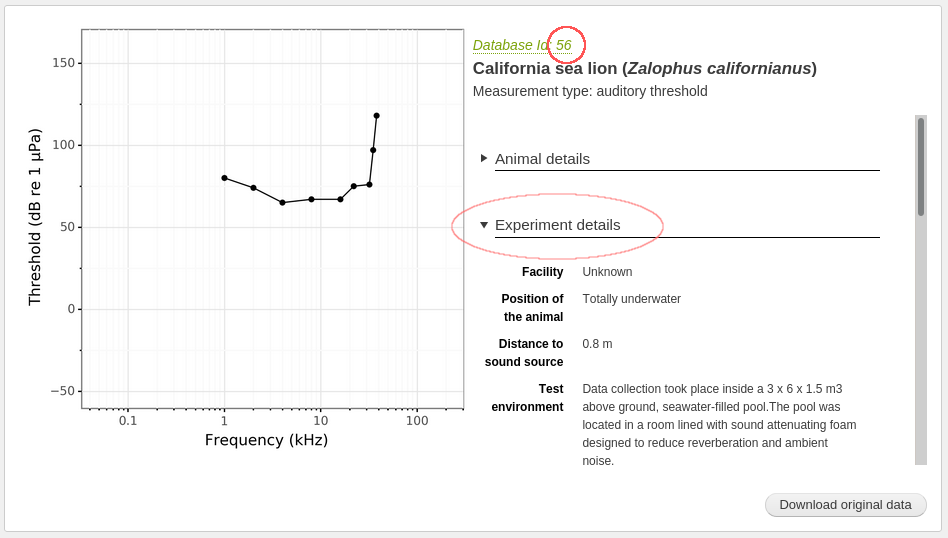
\includegraphics[width=\textwidth]{experiment_details.png}
\caption{Audiogram with open experiment details tab}
\label{fig:experiment_details}
\end{figure}

\begin{it}During editing, it is recommended to open the AAD in a second window. The audiogram used in fig. \ref{fig:experiment_details} is audiogram 56, \url{https://animalaudiograms.museumfuernaturkunde.berlin/audiogram?ids=56}.
\end{it}
\subsection{Experiment details input form}
In the \href{https://animalaudiograms.museumfuernaturkunde.berlin/admin/v1/start}{administrative interface}, click on the ``Edit experiment details'' link. This will open a form that lets you edit the details of an \emph{existing} experiment, i.e. one that is \emph{already in the database}.

To edit an experiment's details, type the audiograms id into the ``Id of an audiogram'' input field. You can find this id in the audiogram's AAD page, at the top of the audiogram display (fig. \ref{fig:experiment_details}).

Using this form you will notice that some input fields receive any input, while some have a predefined list of possible values. These predefined values have been established in expert workshops and are documented in the \href{https://github.com/MfN-Berlin/AnimalAudiogramDatabase/blob/main/resources/metadata/audiogram_metadata_scheme.md}{metadata scheme}.

These details include type of measurement, facility, position of the animal, distance to sound source, test environment, medium, method, calibration, threshold, staircase procedure, method of constants and sedation state of an experiment. 

Additionally, the publication that is the source of this experiment, and the animal this experiment relates to, can be edited (the first 2 input fields).
\begin{itemize}
\item{If the publication required is not yet in the database, please add it using the ``Add a publication'' function explained below}
\item{If the animal species required is not yet in the database, please add it using the ``Add a species detail'' function explained below}
\end{itemize}


% ----------------------------------------------------------------------------------------------%
\section{Edit an animal's details}
\subsection{What are animal details?}
Animal details can be found under the ``Animal details'' tab of each audiogram in the AAD.

\subsection{Animal details input form}
In the \href{https://animalaudiograms.museumfuernaturkunde.berlin/admin/v1/start}{administrative interface}, click on the ``Edit animal details'' link. This will open a form that lets you edit the details of animal associated with an \emph{existing} experiment, i.e. one that is \emph{already in the database}.

To edit an animal's details, type the audiograms id into the ``Id of an audiogram'' input field. You can find this id in the audiogram's AAD page, at the top of the audiogram display (fig. \ref{fig:experiment_details}).

Using this form, you can edit the details of the animal \emph{at the time the animal was involved in the experiment}. These details include species, name of the animal, sex, liberty status, life stage, age of the animal, duration in captivity. 

% ----------------------------------------------------------------------------------------------%
\section{Edit an audiogram's data points}
\subsection{What are data points?}
Data points are the points shown in the graphic representation of an audiogram.

\subsection{Data points form}
In the \href{https://animalaudiograms.museumfuernaturkunde.berlin/admin/v1/start}{administrative interface}, click on the ``Edit an audiogram's data points'' link. This will open a form that lets you edit the data points of an audiogram, i.e. of an audiogram that is \emph{already in the database}. Data points are sorted by frequency. This form also lets you add data points to an existing audiogram (fig. \ref{fig:edit_data_points}).

To edit or add data points to an existing audiogram, type the audiogram's id into the ``Id of an audiogram'' input field. You can find this id in the audiogram's AAD page, at the top of the audiogram display (fig. \ref{fig:experiment_details})

\begin{figure}
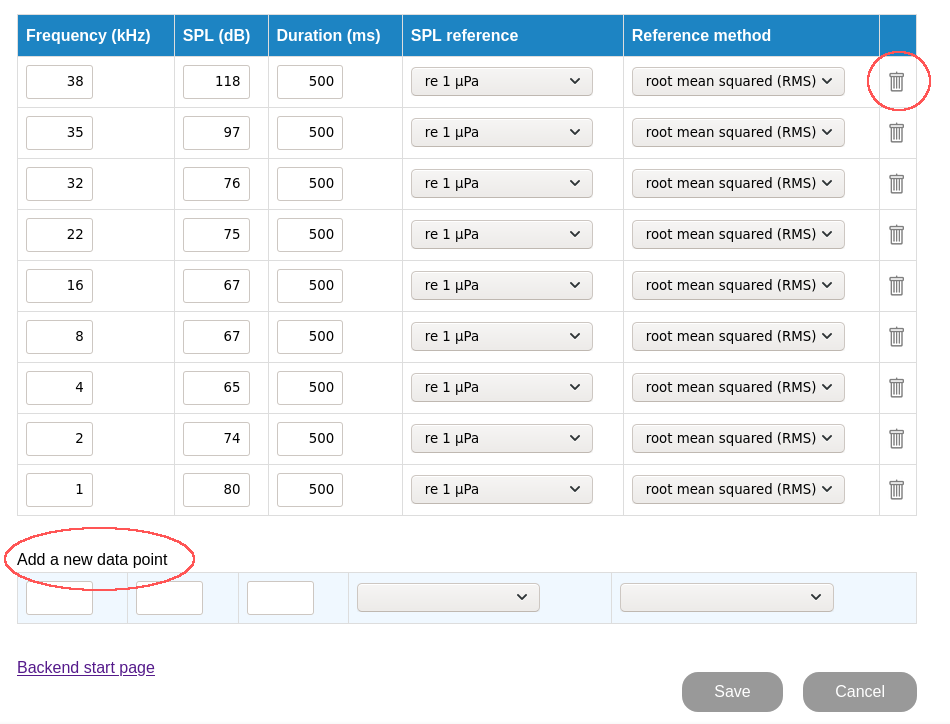
\includegraphics[width=\textwidth]{edit_data_points.png}
\caption{Editing an audiogram's data points}
\label{fig:edit_data_points}
\end{figure}

Each data point represents frequency, sound pressure level (SPL), duration, SPL reference and reference method. Edits (including deletions) will only take effect after the page has been saved.
\begin{itemize}
\item{The values of each data point can be edited individually}
\item{Individual data points can be marked for deletion (fig. \ref{fig:edit_data_points})}
\item{New data points can be added using the last row, which is always empty when the page is loaded}
\end{itemize}


% ----------------------------------------------------------------------------------------------%
\section{Delete an audiogram}
In the \href{https://animalaudiograms.museumfuernaturkunde.berlin/admin/v1/start}{administrative interface}, click on the ``Delete an audiogram'' link. You will be asked to confirm the action. Deleting an audiogram is irreversible.

% ----------------------------------------------------------------------------------------------%
\section{Adding a publication}
Add bibliographical details of a publication (Autors, Title, Journal, DOI, etc.). If the publication is already in the database, skip this step.

Publication details can be retrieved automatically by DOI. To do this, go to the \href{https://animalaudiograms.museumfuernaturkunde.berlin/admin/v1/start}{administrative interface}, click on the ``Add a publication'' link. Input a DOI of a publication and retrieve the data from the \href{https://www.doi.org/}{International DOI Foundation (IDF)}.

The ``citation long'' field shows the complete bibliographic data. The ``citation short'' field shows the citation formatted in \href{https://apastyle.apa.org}{APA style}.

% ----------------------------------------------------------------------------------------------%
\section{Adding a species details}
Add taxonomic details of a new species (Latin name, vernacular name, etc.). If the species is already in the database, skip this step. Taxonomic details can be retrieved automatically from the Tree of Life database.

Species taxonomy: phylum, class, order, family, genus species and unique name, can be retrieved automatically from the \href{https://opentreeoflife.github.io}{Open Tree of Life database}. To retrieve the taxonomy for an animal, input the species' latin name (fig. \ref{fig:taxonomy}).

Taxonomical information does not include the vernacular name. You will have to input the vernacular name yourself (required field).

\ref{fig:experiment_details}).
\begin{figure}
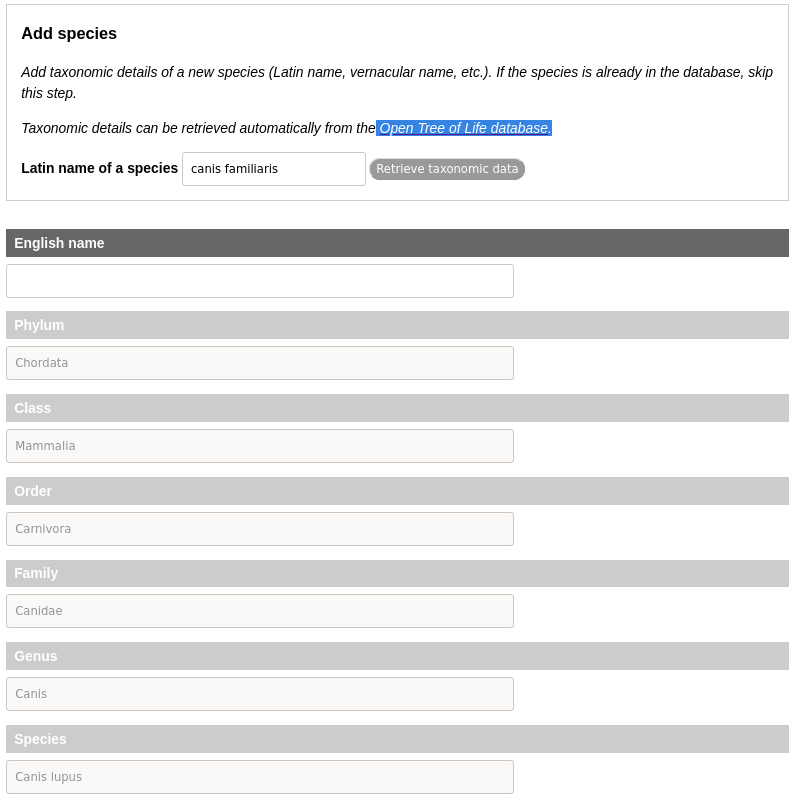
\includegraphics[width=\textwidth]{taxonomy.png}
\caption{Retrieving a taxonomy from Open Tree of Life}
\label{fig:taxonomy}
\end{figure}

% ----------------------------------------------------------------------------------------------%
\section{Add a new experiment to the database}
Create an experiment and add metadata about publication, method, etc.
Adding a new audiogram to the database requires a combination of several actions described above:

\begin{itemize}
\item{If the publication for this audiogram is not listed, then add it first, using the then reload the page.}
\item{If the animal species for this audiogram is not listed, then add it first, then reload the page.}
\item{Create an experiment and add metadata about publication, method, etc., \emph{using this form}}
\item{Finally, open the newly created a experiment and add the audiogram's data points}
\end{itemize}

% ----------------------------------------------------------------------------------------------%
\section{Further documentation}
Audiogram Metadata Scheme
\url{https://github.com/MfN-Berlin/AnimalAudiogramDatabase/blob/main/resources/metadata/audiogram_metadata_scheme.md}
\\\\
Documentation on how to query, use, and view the audiograms in the database:
\url{https://animalaudiograms.museumfuernaturkunde.berlin/How-to}
\\\\
Examples of data analyses using data extracted from the AAD:
\url{https://raw.githubusercontent.com/MfN-Berlin/HIP_audiogramdb_examples/master/usage_examples.pdf}
\\\\
Source code and technical documentation on how to setup the database: \url{https://github.com/MfN-Berlin/AnimalAudiogramDatabase}

\end{document}


